\lecturechapter{Monday}{Feb 23rd}{February 23rd 2026}{Topology of Metric Spaces}

\begin{nice-box}[Context]
This lecture transitions from the basic definitions of metric spaces and sequences to the study of \emph{Topology}. The lecturer, Joaquim Serra, introduces the fundamental concepts of open and closed sets, interior, and closure. These concepts provide the language necessary to discuss continuity and limits in a more abstract and powerful framework, moving beyond the specific Euclidean structure of $\mathbb{R}^n$.
\end{nice-box}

\begin{meta-note}[Initial Board State]
The left chalkboard contains a summary of previous lectures:
\begin{itemize}
    \item $(X, d)$ metric space [$\mathbb{R}^n, d_{\text{Eucl}}$]
    \item $(x_n)_{n \ge 0} \quad x_n \to x$
    \item Cauchy seq. $\mid$ Complete metric space
\end{itemize}
Below this, the plan for today is written:
\begin{itemize}
    \item Today: Open \& closed sets
    \item Continuous functions
\end{itemize}
\end{meta-note}

% ==========================================
% SECTION 1: RECALL AND MOTIVATION
% ==========================================
\section{Recall and Motivation}

\begin{spoken-clean}[00:00:00 - 00:01:50]
We can continue. Uh, good afternoon. We can --- we can continue where we left it last time. So, I remind --- so just a quick summary of what we saw the last lectures. First lecture was mostly introduction, but then we saw metric spaces. And I told you --- because people already asked me, even though I thought the first day --- why we studied metric spaces. So, the model --- whenever it gets too abstract, the model you need to have in mind all the time for this $(X, d)$ metric space is $\mathbb{R}^n$ with the Euclidean distance, okay? So, whenever you have doubts, just plug $\mathbb{R}^n$ where there is an $X$ (a capital $X$) and $d$ is the usual --- the modulus of the difference of the points. 

And, uh, I said that I wanted to do this in this more general framework because later, in the last part of the course, we will use other spaces, okay? And for good reason. It's not --- I mean, we will use to prove some theorems in the course, the space of continuous functions. But, uh, if you want, for the --- this is not something that belongs to mathematicians, right? Let me say very quickly for the physicists: so, in classical mechanics, the points in the space is a vector in $\mathbb{R}^n$, right? But when you will go to quantum mechanics, what is a point? What is the position of a particle in space? Is the wave function. This is a function. So, the functions, the wave functions, are naturally points in your space, right? So, this is what we are saying here. We are trying to say things more general to be able to understand, um, the things that come naturally in the physics, for instance.
\end{spoken-clean}

\begin{spoken-clean}[00:01:50 - 00:02:22]
Okay. So, now, in this framework of metric spaces, we saw what it means a sequence, what it means that a sequence converges, what is a Cauchy sequence, what is a complete metric space, and we proved that $\mathbb{R}^n$ is always a complete metric space using that $\mathbb{R}$ is complete, this last time. And today we will see the definition of open and closed sets in a metric space and the notion of continuous functions in the setup of metric spaces. So, let me start with the definition of open ball.
\end{spoken-clean}

% ==========================================
% SECTION 2: OPEN BALLS AND OPEN SETS
% ==========================================
\section{Open Balls and Open Sets}

\begin{math-stroke}[Definition: Open Ball]
\setcounter{section}{2} \setcounter{subsection}{0} \setcounter{theorem}{37}
\begin{definition}[Open Ball]\label{def:open-ball-v2}
Let $(X, d)$ be a metric space. We define the \emph{open ball} of radius $r > 0$ centered at a point $x \in X$ as the set:
\[ B(x, r) = \{ y \in X \mid d(y, x) < r \} \]
\end{definition}

\begin{explanation-of-steps}
The open ball consists of all points in the space whose distance to the center $x$ is strictly less than the radius $r$. The strict inequality is what makes the ball \qt{open}—it does not include its boundary.
\end{explanation-of-steps}

\begin{ai-note}[Notation]
The lecturer notes that an equivalent notation often found in literature is $B_r(x)$.
\end{ai-note}
\end{math-stroke}

\begin{spoken-clean}[00:03:54 - 00:04:51]
So, if you want a drawing of that, in the Euclidean space --- in a general metric space I cannot draw anything because it's too general, but in the Euclidean space, let's say in $\mathbb{R}^2$, the metric ball would be the ball. So, the --- the open ball would be this, right? \inlinemetanote{Draws a circle on the board} What is inside of the --- of the ball. And it's open because you don't include --- if you want I can --- I can put the boundary of the ball, that we will introduce today also in a general topological space what the boundary means. This surface of the ball is not included, because there is a strict inequality. The points that are at exactly distance $r$, I don't take them. This is the open ball.
\end{spoken-clean}

\begin{math-stroke}[Visualizing the Open Ball in \texorpdfstring{$\mathbb{R}^2$}{R2}]
\begin{center}
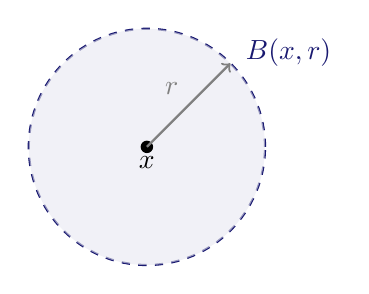
\begin{tikzpicture}[scale=1.5]
% \begin{ai-tikz-planner-invisible-content}
% 1. Background: A point x.
% 2. Midground: A dashed circle representing the boundary.
% 3. Foreground: Shaded interior representing the open ball.
% \end{ai-tikz-planner-invisible-content}
    \coordinate (X) at (0,0);
    \draw[dashed, thick, MidnightBlue] (X) circle (1cm);
    \fill[MidnightBlue!10, opacity=0.6] (X) circle (1cm);
    \fill (X) circle (1.5pt) node[below] {$x$};
    \draw[->, thick, gray] (X) -- (0.707, 0.707) node[midway, above left] {$r$};
    \node[MidnightBlue] at (1.2, 0.8) {$B(x, r)$};
\end{tikzpicture}
\end{center}
\end{math-stroke}

\begin{spoken-clean}[00:04:51 - 00:05:52]
Now, next definition is open and closed sets. \inlinemetanote{Writes on the board} So, we say that a set $U$ of my metric space $X$ is open if for every $x$ in $U$, exists some positive radius $r$ (depending on $x$, possibly) such that the ball of radius $r$ centered at $x$ is contained in $U$.
\end{spoken-clean}

\begin{math-stroke}[Definition: Open and Closed Sets]
\setcounter{theorem}{38}
\begin{definition}[Open and Closed Sets]\label{def:open-closed-sets}
Let $(X, d)$ be a metric space.
\begin{itemize}
    \setcounter{enumi}{0} \item A subset $U \subseteq X$ is \emph{open} if every point in $U$ is the center of some open ball entirely contained within $U$:
    \[ \forall x \in U, \exists r > 0 \text{ s.t. } B(x, r) \subseteq U \]
    \setcounter{enumi}{1} \item A subset $A \subseteq X$ is \emph{closed} if its complement is open:
    \[ A \text{ is closed} \iff X \setminus A \text{ is open} \]
\end{itemize}
\end{definition}
\end{math-stroke}

% \begin{ai-global-state-checkpoint-invisible-content}
% timestamp: 00:06:00
% topic: Definitions of open balls, open sets, and closed sets.
% board_state: def:open-ball, def:open-closed-sets
% next_goal: Provide geometric intuition for open sets.
% open_loops: none
% \end{ai-global-state-checkpoint-invisible-content}

\begin{spoken-clean}[00:05:52 - 00:07:10]
So, I will draw some in $\mathbb{R}^2$ some open set. Is essentially any set --- this is a bit heuristically, this is the idea, right? Then we will see concrete open sets. But it's a set that doesn't --- does not include its contour, so its boundary. Again, I didn't define the boundary yet, but now you know --- you have some common sense knowledge of what is a boundary of this set, that is this part --- the skin of the set, right? If the set is the inside without the skin, this is open. Why? Because any point here, you can take a ball, depending on the distance to the boundary, right? Depending on the distance to the skin, you make the ball super small and it will be contained in the set. It's like I said: any point in the interior will be at positive distance from the skin.
\end{spoken-clean}

\begin{math-stroke}[Intuition for Open Sets]
\begin{center}
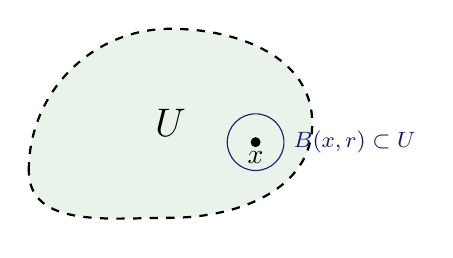
\begin{tikzpicture}[scale=1.2]
% \begin{ai-tikz-planner-invisible-content}
% 1. Background: A generic blob with a dashed boundary.
% 2. Midground: A point x near the boundary.
% 3. Foreground: A small ball B(x, r) contained within the blob.
% \end{ai-tikz-planner-invisible-content}
    % The Open Set U
    \draw[dashed, thick, fill=ForestGreen!10] 
        (0,0) to[out=90,in=180] (1.5,1.5) 
        to[out=0,in=90] (3,0.5) 
        to[out=-90,in=0] (1.5,-0.5) 
        to[out=180,in=-90] cycle;
    \node at (1.5, 0.5) {\Large $U$};

    % Point x and its ball
    \coordinate (X) at (2.4, 0.3);
    \fill (X) circle (1.5pt) node[below] {$x$};
    \draw[MidnightBlue] (X) circle (0.3cm);
    \node[MidnightBlue, right] at (2.7, 0.3) {\footnotesize $B(x, r) \subset U$};
\end{tikzpicture}
\end{center}
\begin{explanation-of-steps}
The \qt{skin} or boundary of an open set is not part of the set itself. This ensures that no matter how close a point $x$ is to the edge, there is always a tiny bit of \qt{breathing room} around it that remains entirely within $U$.
\end{explanation-of-steps}
\end{math-stroke}

\begin{spoken-clean}[00:07:10 - 00:08:37]
So, if you want a more concrete example, take the set $(0, 1) \times (0, 1)$, the square, open square, subset $\mathbb{R}^2$. This --- prove that it is open. Exercise. So, you take this square... \inlinemetanote{Draws a dashed square on the board} You take a point here. A point in the square will have two coordinates. And now, what is the definition of open? If you take the point, this point is $(x_1, x_2)$, you need to find a radius $r$ positive such that the whole ball centered at this given point belongs to the square. In the case of the square, what is the formula for the radius? Well, you can take $r$ equal, I don't know, something like the minimum between this distance, this distance, this distance, and this distance. So, it will be something like the minimum between $x_1, x_2, 1 - x_1$ and $1 - x_2$. You can check that this radius works. The minimum of these four numbers.
\end{spoken-clean}

\begin{math-stroke}[Example: The Open Unit Square]
Consider the open unit square in $\mathbb{R}^2$:
\[ U = (0, 1) \times (0, 1) = \{ (x_1, x_2) \in \mathbb{R}^2 \mid 0 < x_1 < 1, 0 < x_2 < 1 \} \]
\begin{center}
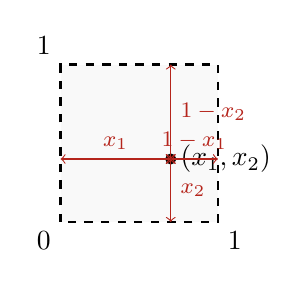
\begin{tikzpicture}[scale=2]
    % Square
    \draw[dashed, thick, fill=gray!5] (0,0) rectangle (1,1);
    \node[below left] at (0,0) {$0$};
    \node[below right] at (1,0) {$1$};
    \node[above left] at (0,1) {$1$};

    % Point x
    \coordinate (X) at (0.7, 0.4);
    \fill (X) circle (1pt) node[right] {$(x_1, x_2)$};
    
    % Distances to boundaries
    \draw[<->, BrickRed] (0.7, 0) -- (0.7, 0.4) node[midway, right] {\footnotesize $x_2$};
    \draw[<->, BrickRed] (0, 0.4) -- (0.7, 0.4) node[midway, above] {\footnotesize $x_1$};
    \draw[<->, BrickRed] (0.7, 0.4) -- (1, 0.4) node[midway, above] {\footnotesize $1-x_1$};
    \draw[<->, BrickRed] (0.7, 0.4) -- (0.7, 1) node[midway, right] {\footnotesize $1-x_2$};
\end{tikzpicture}
\end{center}
\begin{explanation-of-steps}
To prove $U$ is open, for any $(x_1, x_2) \in U$, we choose the radius:
\[ r = \min(x_1, x_2, 1 - x_1, 1 - x_2) \]
Since $0 < x_1, x_2 < 1$, all four values are strictly positive, so $r > 0$. The ball $B((x_1, x_2), r)$ is then guaranteed to be contained within the square.
\end{explanation-of-steps}
\end{math-stroke}

\begin{spoken-clean}[00:08:37 - 00:10:16]
Okay, second point in the definition is what is a closed set. \inlinemetanote{Writes on the board} So, $A$ subset $X$ is called closed if the complement is open: $X \setminus A$ is open. So, now, this set --- this set is not closed, you can show. Instead, this set... \inlinemetanote{Writes $[0, 1] \times [0, 1]$ on the board} for instance, this set is closed. Now it needs to contain the skin to be closed. Because then, when you pass to the complement, that is by definition open, it need not to contain the boundary. So, the closed sets, we draw them with their skin.
\end{spoken-clean}

\begin{math-stroke}[Example: The Closed Unit Square]
The closed unit square is defined as:
\[ A = [0, 1] \times [0, 1] = \{ (x_1, x_2) \in \mathbb{R}^2 \mid 0 \le x_1 \le 1, 0 \le x_2 \le 1 \} \]
\begin{center}
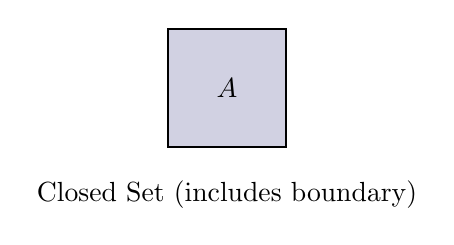
\begin{tikzpicture}[scale=1.5]
    \draw[thick, fill=MidnightBlue!20] (0,0) rectangle (1,1);
    \node at (0.5, 0.5) {$A$};
    \node[below] at (0.5, -0.2) {Closed Set (includes boundary)};
\end{tikzpicture}
\end{center}
\begin{explanation-of-steps}
The set $A$ is closed because its complement, $\mathbb{R}^2 \setminus A$, is open. If you take any point outside the closed square, there is a minimum distance to the square's boundary, allowing you to fit a small open ball around that point that does not touch $A$.
\end{explanation-of-steps}
\end{math-stroke}

% \begin{ai-global-state-checkpoint-invisible-content}
% timestamp: 00:12:00
% topic: Definitions of open/closed sets and the concept of topology.
% board_state: def:open-closed-sets, ex:open-square, ex:closed-square
% next_goal: Define the topology associated with a metric.
% open_loops: none
% \end{ai-global-state-checkpoint-invisible-content}

\begin{spoken-clean}[00:10:16 - 00:11:35]
Okay, maybe this I can erase. And maybe the last part of this definition, that you will not use --- we will not use actually, but --- but is something that is a common term that you will find in books and it's good that we know, is what is the topology. So, you will see in the notes you will see the word topology many times. You are not yet studying topology, but --- just for information, the word topology, topology associated to the distance $d$ is the --- we can put a $\mathcal{T}$ like this, a sort of calligraphic $\mathcal{T}$, is the collection of all the open sets. This is the topology. So, when we say that something is a topological notion, it has to do with this collection of open sets.
\end{spoken-clean}

\begin{math-stroke}[The Topology of a Metric Space]
\begin{definition}[Topology]\label{def:topology-v2}
The \emph{topology} $\mathcal{T}$ associated with a metric space $(X, d)$ is the collection of all open subsets of $X$:
\[ \mathcal{T} = \{ U \subseteq X \mid U \text{ is open} \} \]
\end{definition}
\end{math-stroke}

% ==========================================
% SECTION 3: PROPERTIES OF OPEN SETS
% ==========================================
\section{Properties of Open Sets}

\begin{spoken-clean}[00:11:35 - 00:13:43]
Now, to see a bit more what are --- because this is still a bit abstract --- to see a bit more practically how we identify open and closed sets, we are going to do it through sequences. Well, let me first do a lemma, maybe, that we will use many times. Lemma: unions and intersections of open sets. This is one of the basic properties. It's very simple, but since we will use many, many times, I prove it now. So, it says that if you have --- I will put it with words and then we will prove with symbols. So, arbitrary unions of open sets are open. This means that if you have some collection $\{U_i\}_{i \in I}$ of $U_i \subseteq X$ open, then the union of this collection (that can be the union of the collection) is also open. Right?
\end{spoken-clean}

\begin{nice-box}[Proposition: Unions and Intersections of Open Sets]
\setcounter{theorem}{42}
\begin{proposition}[Unions and Intersections of Open Sets]
  \label[proposition]{prop:open-sets-properties}
In any metric space $(X, d)$:
\begin{enumerate}
    \setcounter{enumi}{0} \item \emph{Arbitrary Unions:} The union of any collection of open sets is open.
    \label[proposition]{prop:open-sets-properties:1:arbitrary-unions}
    \setcounter{enumi}{1} \item \emph{Finite Intersections:} The intersection of a finite number of open sets is open. 
    \label[proposition]{prop:open-sets-properties:2:finite-intersections}
\end{enumerate}
\end{proposition}
\end{nice-box}

\begin{proof}[Proof of Proposition \ref{prop:open-sets-properties} (Part 1)]
\begin{spoken-clean}[00:13:43 - 00:15:50]
And also finite intersections of open sets are open. Right? So, this means that if $I$ is finite, the intersection --- let's say, let's put it like this: the intersection of $U_i$ for $i$ between $1$ and capital $N$, a bounded number, this is open set. 

The proof of this is just using the definition. So, if I want to check that a union is open, I take a point $x$ in this set that is the union. Let me call this in the union. Right? And then, in particular, $x$ belongs to one of them because it's a union. I call $i_0$ is one of the $i$s. I fix any of them. And then, since this one is open, exists some radius $r$ such that the ball of radius $r$ centered at $x$ is contained in $U_{i_0}$. But this is contained in the union. Which proves that this union is open, right?
\end{spoken-clean}

\begin{math-stroke}[Proof: Arbitrary Unions]
Let $\{U_i\}_{i \in I}$ be a collection of open sets. Let $U = \bigcup_{i \in I} U_i$.
Take any point $x \in U$. By the definition of union:
\[ x \in U \implies \exists i_0 \in I \text{ s.t. } x \in U_{i_0} \]
Since $U_{i_0}$ is open, by definition:
\[ \exists r > 0 \text{ s.t. } B(x, r) \subseteq U_{i_0} \]
Since $U_{i_0} \subseteq \bigcup_{i \in I} U_i = U$, it follows that:
\[ B(x, r) \subseteq U \]
Thus, $U$ is open.
\end{math-stroke}
\end{proof}

% \begin{ai-global-state-checkpoint-invisible-content}
% timestamp: 00:18:00
% topic: Properties of open sets and student interaction on "clopen" sets.
% board_state: prop:open-sets-properties, proof:unions
% next_goal: Address student question about sets that are both open and closed.
% open_loops: none
% \end{ai-global-state-checkpoint-invisible-content}

\begin{student-interaction}[Student Question]
Except for the empty set and the set $X$ itself, can you give us some examples of both closed and open sets?
\end{student-interaction}

\begin{spoken-clean}[00:18:16 - 00:19:15]
We will discuss this when we --- when we discuss connected spaces. Okay? This is a good question. So, the --- the whole space and the empty set are always open and closed, and I will emphasize this when we see connected spaces. So, you need to wait a bit more. I could give an example, but it's not very interesting. It's just a disconnected space like the union, the disjoint union of two intervals or something like that, then each interval is open and closed. But this will not be very interesting. You will see the interest of this question when we see connected spaces. Okay? But it's a fair question.
\end{spoken-clean}

\begin{didactic-insight}[Clopen Sets and Connectivity]
The lecturer hints at a deep topological property: in a \qt{connected} space (like $\mathbb{R}^n$), the only sets that are both open and closed (often called \qt{clopen}) are the empty set and the space itself. The existence of other clopen sets is the defining characteristic of a disconnected space.
\end{didactic-insight}

% ==========================================
% SECTION 4: PROPERTIES OF CLOSED SETS
% ==========================================
\section{Properties of Closed Sets}

\begin{spoken-clean}[00:19:15 - 00:21:15]
So, I am saying that when you take open sets, when you take finitely many intersections of open sets, you get something open. Why? I will say with words and then you try to write down, okay? So, you have finitely many open sets. And now you take a point that is in the intersection of these finitely many. This means that the point is in all of them. And now, for each of the sets, you pick a radius that is different in every time. But there are finitely many radii that you can put your ball in the open set. And if you take the minimum of all these radii, it will be good. With the minimum of the finitely many radii, you will fall inside of the intersection. Okay? You don't need to understand what I said, please try to do the exercise. If there are problems doing this, you have it in the notes. But I think this is a very good opportunity to do as an exercise to see if we understood the definitions. Because it's one line, so it's not --- you don't need to think too much.
\end{spoken-clean}

\begin{math-stroke}[Proof Sketch of \cref{prop:open-sets-properties} \labelcref{prop:open-sets-properties:2:finite-intersections}: Finite Intersections of Open Sets]
\begin{ai-proof-skeleton-invisible-content}
% 1. Take x in the intersection of U_1, ..., U_N.
% 2. For each i, x is in U_i, so there exists r_i > 0 s.t. B(x, r_i) is in U_i.
% 3. Let r = min(r_1, ..., r_N). Since N is finite, r > 0.
% 4. Then B(x, r) is in B(x, r_i) for all i, so B(x, r) is in the intersection.
\end{ai-proof-skeleton-invisible-content}
\begin{short-proof}[Proof Sketch]
Let $U = \bigcap_{i=1}^N U_i$ where each $U_i$ is open. Take $x \in U$.
Then $x \in U_i$ for all $i \in \{1, \dots, N\}$. Since each $U_i$ is open:
\[ \forall i, \exists r_i > 0 \text{ such that } B(x, r_i) \subseteq U_i \]
Let $r = \min(r_1, r_2, \dots, r_N)$. Because we are taking the minimum of a \emph{finite} set of positive numbers, $r > 0$.
Then for all $i$, $B(x, r) \subseteq B(x, r_i) \subseteq U_i$.
Therefore, $B(x, r) \subseteq \bigcap_{i=1}^N U_i = U$, proving that $U$ is open.
\end{short-proof}
\end{math-stroke}

\begin{spoken-clean}[00:21:15 - 00:24:04]
Okay. Now, analogous lemma but for closed sets. \inlinemetanote{Writes on the board} Unions and intersections of closed sets. And it's the same but the opposite. So, it says that finite unions of closed sets are closed and arbitrary intersections of closed sets are closed. And the proof is --- well, you can repeat the same proof or you can reason a bit more --- or a variant of the same proof, or you can reason passing to the complement. So, you can use that being closed is defined as the complement being open. So, if you pass to the complement, the complementation converts closed sets in open and open in closed. So, you can always pass statements about open sets to the complement and you get a statement about closed sets. And this is what we have here. Why? Because $X$ minus a union of sets is the same as the intersection of the complements. Right? So, when you do the complement of a union, you get the intersection of the complements. And the same, the complement of a intersection is equal to the union of the complements. And then you apply the previous result. Because if these sets are closed, these sets will be open, and the finite intersection of open is open.
\end{spoken-clean}

\begin{nice-box}[Lemma: Unions and Intersections of Closed Sets]
\setcounter{theorem}{43}
\begin{proposition}[Unions and Intersections of Closed Sets]\label{prop:closed-sets-properties}
In any metric space $(X, d)$:
\begin{enumerate}
    \setcounter{enumi}{0} \item \emph{Finite Unions:} The union of a finite number of closed sets is closed.
    \setcounter{enumi}{1} \item \emph{Arbitrary Intersections:} The intersection of any collection of closed sets is closed.
\end{enumerate}
\end{proposition}
\end{nice-box}

\begin{math-stroke}[Proof via De Morgan's Laws]
The properties of closed sets follow directly from those of open sets using De Morgan's Laws:
\begin{align*}
X \setminus \left( \bigcup_{i \in I} A_i \right) &= \bigcap_{i \in I} (X \setminus A_i) \\
X \setminus \left( \bigcap_{i \in I} A_i \right) &= \bigcup_{i \in I} (X \setminus A_i)
\end{align*}
\begin{explanation-of-steps}
If each $A_i$ is closed, then each complement $(X \setminus A_i)$ is open. 
\begin{itemize}
    \item For an arbitrary intersection $\bigcap A_i$, its complement is the union $\bigcup (X \setminus A_i)$. Since the arbitrary union of open sets is open, the intersection is closed.
    \item For a finite union $\bigcup_{i=1}^N A_i$, its complement is the finite intersection $\bigcap_{i=1}^N (X \setminus A_i)$. Since the finite intersection of open sets is open, the union is closed.
\end{itemize}
\end{explanation-of-steps}
\end{math-stroke}

% \begin{ai-global-state-checkpoint-invisible-content}
% timestamp: 00:24:00
% topic: Properties of closed sets and the importance of finiteness.
% board_state: prop:closed-sets-properties, eq:de-morgan
% next_goal: Show an example where infinite intersection of open sets is not open.
% open_loops: none
% \end{ai-global-state-checkpoint-invisible-content}

\begin{spoken-clean}[00:24:04 - 00:26:39]
Let me give some example, very easy, that this property when we said finite intersections or finite unions is important that it is finite. That when you get infinite intersections of open sets, you can get a closed set that is not open. So, example: finite is important. So, if you take the simplest --- well, one of the spaces that you are most familiar with that is $\mathbb{R}$ with the Euclidean distance, and you take the sets $U_k = (-1/k, 1/k)$. And you take its intersection, then the intersection for $k=1$ to infinity of $U_k$, this gives you the point $\{0\}$. So, these are open intervals, and it's very easy because the intervals do not contain the endpoints, each of them is open. But when you do their intersection, you get just the point zero, and the point zero is not open because you cannot put any ball that contains anything. The point zero is closed but is not open. So, these are open and this is not open! That's why it's important that the intersection is finitely many. And passing to the complement you get a counterexample for the infinite unions of closed sets.
\end{spoken-clean}

\begin{math-stroke}[Example: Infinite Intersection of Open Sets]
\setcounter{theorem}{44}
\begin{example}[Infinite Intersection of Open Sets]\label{ex:infinite-intersection}
Consider the metric space $(\mathbb{R}, d_{\text{Eucl}})$. Define a sequence of open intervals:
\[ U_k = \left( -\frac{1}{k}, \frac{1}{k} \right) \quad \text{for } k \in \{1, 2, 3, \dots\} \]
Each $U_k$ is an open set. However, their infinite intersection is:
\[ \bigcap_{k=1}^{\infty} U_k = \{0\} \]
\begin{center}
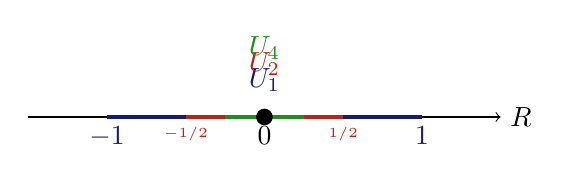
\begin{tikzpicture}[scale=2]
    \draw[->] (-1.5,0) -- (1.5,0) node[right] {$\mathbb{R}$};
    \draw[ultra thick, MidnightBlue] (-1,0) -- (1,0);
    \node[below, MidnightBlue] at (-1,0) {$-1$};
    \node[below, MidnightBlue] at (1,0) {$1$};
    \node[above, MidnightBlue] at (0, 0.1) {$U_1$};

    \draw[ultra thick, BrickRed] (-0.5,0) -- (0.5,0);
    \node[below, BrickRed] at (-0.5,0) {\tiny $-1/2$};
    \node[below, BrickRed] at (0.5,0) {\tiny $1/2$};
    \node[above, BrickRed] at (0, 0.2) {$U_2$};

    \draw[ultra thick, ForestGreen] (-0.25,0) -- (0.25,0);
    \node[above, ForestGreen] at (0, 0.3) {$U_4$};
    
    \fill[black] (0,0) circle (1.5pt) node[below] {$0$};
\end{tikzpicture}
\end{center}
\begin{explanation-of-steps}
As $k \to \infty$, the intervals shrink around the origin. The only point contained in \emph{every} interval is $0$. The set $\{0\}$ is a singleton set, which is closed in $\mathbb{R}$ but not open, as any open ball $B(0, r) = (-r, r)$ contains points other than $0$.
\end{explanation-of-steps}
\end{example}
\end{math-stroke}

% ==========================================
% SECTION 5: INTERIOR AND CLOSURE
% ==========================================
\section{Interior and Closure}

\begin{spoken-clean}[00:26:39 - 00:28:30]
Okay, so now we will define something interesting that is what we were saying there heuristically: so what is the interior and the boundary of a set in a metric space. So, given a set $\Omega$ in my metric space $X$, I define the interior of $\Omega$. This is called the interior of $\Omega$. This is by definition the largest open set contained in $\Omega$. So, you have your set $\Omega$ and you look at all the open sets that are contained and you get the largest one is the union of all the open sets that contain $\Omega$. This is the interior.
\end{spoken-clean}

\begin{math-stroke}[Definition: Interior and Closure]
\setcounter{theorem}{45}
\begin{definition}[Interior and Closure]\label{def:interior-closure}
Let $(X, d)$ be a metric space and $\Omega \subseteq X$ be any subset.
\begin{itemize}
    \setcounter{enumi}{0} \item The \emph{interior} of $\Omega$, denoted $\operatorname{int}(\Omega)$ or $\Omega^\circ$, is the largest open set contained in $\Omega$. Formally, it is the union of all open subsets of $\Omega$:
    \[ \operatorname{int}(\Omega) = \bigcup \{ U \subseteq \Omega \mid U \text{ is open} \} \]
    \item The \emph{closure} of $\Omega$, denoted $\overline{\Omega}$, is the smallest closed set containing $\Omega$.
\end{itemize}
\end{definition}
\end{math-stroke}

\begin{spoken-clean}[00:28:30 - 00:29:59]
Now, I also define the closure, that you know from $\mathbb{R}$, the closure of some set is the set of points $x$ in $X$ such that there exists some sequence $x_n$ such that the whole sequence... \textit{[Audio cuts off abruptly]}
\end{spoken-clean}

\begin{math-stroke}[Sequential Characterization of Closure]
A point $x \in X$ belongs to the closure $\overline{\Omega}$ if and only if it can be reached as the limit of a sequence of points from $\Omega$:
\[ \overline{\Omega} = \{ x \in X \mid \exists (x_n)_{n \ge 0} \subseteq \Omega \text{ s.t. } x_n \to x \} \]
\textit{[Audio cuts off abruptly]}
\end{math-stroke}

% [SYSTEM] Video complete.